\section{Introduction}
Navigating through an environment is one of the fundamental tasks in mobile robotics. For robots with relatively reasonable dynamics and operating speeds in indoor environments, efficient collision-free navigation is practically solved. However, introducing constraints other than ``please take the shortest path without running into anything'' is still an ongoing area of research, especially when taking the social needs of humans into account. These constraints often take the form of non-lethal obstacles, or places that are undesirable to be but do not result in a collision. Modeling non-lethal obstacles in the space around a person will help robots to not invade the person's personal space. 

These representations raise the value of a set of cells in the costmap, making it less likely for the robot to travel in them. In the person-avoiding scenario, this means that the robot will respect the person's personal space more often, since the areas closest to the person will have the highest costs.

However, it is not always the case though that higher costs result in the robot not traveling through a given cell. The robot still could drive through a person's intimate social space given the right circumstances. Such a path would be inoptimal when considering the person's proxemic concerns, but it is still valid and non-lethal (i.e. does not result in a collision). Sometimes this behavior corresponds with the proxemically inoptimal path being the only path available. However, sometimes it results from improperly tuned parameters. While the previous researchers have all tuned their parameters to create working configurations, there exists no general guide for understanding the process of how the parameters change the robot behavior. Furthermore, as our exploration of this space shows, the behavior is not always readily intuitive. 

This paper aims to explore the space of these paths through non-lethal costmaps. 


\begin{figure}
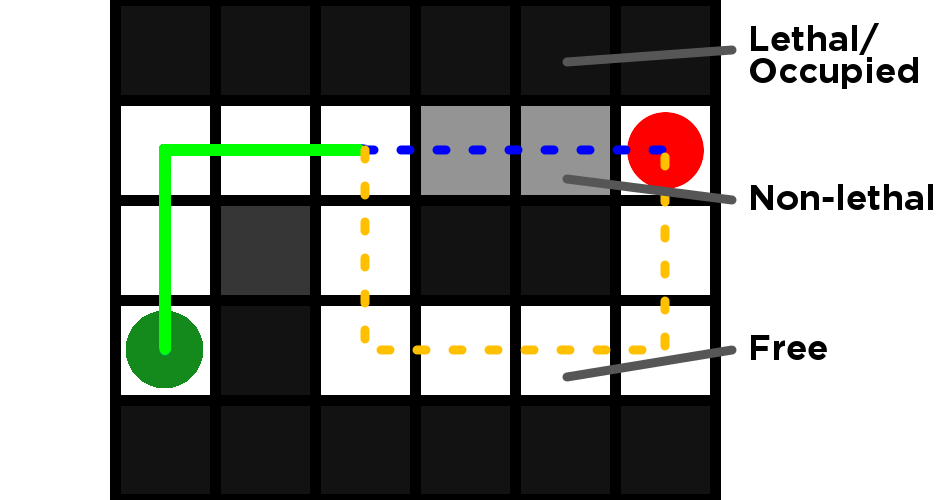
\includegraphics[width=\columnwidth]{graphix/Intro.png}
\caption{Simple Costmap with Non-lethal Obstacles -  In a costmap, the world is discretized into cells. Each cell has a value $f(x,y)$. If the value is greater than some limit $L$, they are considered ``lethal'', meaning that there is an obstacle somewhere in that cell, and entering it will result in a ``lethal'' collision. Cells with a value of zero are considered free, i.e. there is no penalty for entering the cell. Everything in between is a ``non-lethal'' obstacle, meaning there is some reason not to be in the cell, but it won't cause a collision. The robot could either continue along the blue path (the shortest path), or it could take a longer yellow path but avoid the non-lethal obstacle. Which path is optimal and which is the path less traveled depends on how the costmap \emph{and} the path planner are configured. }
\label{fig:intro}
\end{figure}
